\documentclass[10pt]{article}

\usepackage[margin=1in]{geometry}
\usepackage{graphicx}
\usepackage{booktabs}
\usepackage{amsmath}
\usepackage{amssymb}
\usepackage{hyperref}
\usepackage{xcolor}
\usepackage{enumitem}
\usepackage{caption}
\usepackage{subcaption}
\usepackage[numbers]{natbib}
\usepackage{float}
\usepackage{algorithm}
\usepackage{algorithmic}

\hypersetup{
  colorlinks=true,
  linkcolor=blue!60!black,
  citecolor=blue!60!black,
  urlcolor=blue!60!black
}

\title{Adaptive Environment Selection for RL-Based LLM Post-Training}
\author{DSAA3053 Course Project}
\date{April 28, 2026}

\begin{document}
\maketitle

\begin{abstract}
Reinforcement-learning post-training for large language models often mixes heterogeneous environments whose difficulty and usefulness vary over training. Uniform sampling ignores this nonstationarity. This paper studies Adaptive Environment Selection (AES), an online curriculum mechanism that clusters Math and Zebra prompts by difficulty, samples clusters with an Upper Confidence Bound (UCB)-style policy, and periodically refines clusters through conservative micro-bucket re-bucketing. AES is implemented on top of a DUMP/verl GRPO training path. Current evidence supports a modest but useful conclusion: AES produces interpretable adaptive bucketing behavior and selective gains on the Math+Zebra setting. A no-rebucket scheduler improves step-200 validation accuracy over random sampling on both Math and Zebra, and its UCB scores drift from low-index to high-index clusters over training, showing that the sampler is active rather than fixed. Re-bucketing further reveals meaningful structural correction, but also task-composition drift. These results suggest that learner-state-aware environment selection is promising, while accuracy-based initialization and stricter evaluation remain necessary next steps.
\end{abstract}

\section{Introduction}

RL-based LLM post-training increasingly relies on heterogeneous mixtures of tasks, datasets, and difficulty levels. This project focuses on a two-source mixture: Math problems and Zebra logic puzzles. Sampling these environments uniformly is simple, but it assumes that every distribution is equally useful at every point in training. This assumption is unlikely to hold: some distributions may be already solved, some may be too difficult to provide useful gradient signal, and some may become useful only after the model reaches an intermediate competence level.

This project follows the \emph{Algorithm Development} track in the course guideline. The algorithmic contribution is an adaptive environment-selection module for RL-based LLM post-training. The evaluation contribution is a numerical benchmark and diagnostic analysis comparing random sampling, AES sampling, and re-bucketing variants on the checked-in Math+Zebra results.

Curriculum learning argues that example order and difficulty can affect optimization \citep{bengio2009curriculum}. Recent work such as DUMP extends this view to RL-based LLM post-training by using advantage magnitude as a distribution-level learnability signal and UCB as an adaptive scheduling rule \citep{wang2025dump}. This project asks whether a related idea can be made practical in a Math+Zebra reasoning setting: can online advantage signals guide environment selection and correct imperfect static difficulty buckets?

We implement and evaluate Adaptive Environment Selection (AES). AES maintains ordered difficulty clusters, samples clusters using UCB with a probability floor, tracks per-sample decayed absolute advantage, and periodically performs low-frequency neighbor-only re-bucketing. The design intentionally prioritizes interpretability and guardrails over aggressive dynamic reclustering.

The main contribution of this project is not a claim of uniform performance improvement. Instead, the contribution is a repo-backed analysis of where adaptive environment selection already works and where it fails. The strongest current evidence is structural: AES changes sampling and bucket composition in interpretable ways. The downstream performance evidence is mixed, which motivates accuracy-based initialization and stricter evaluation.

\section{Background}

\paragraph{Curriculum learning.}
Curriculum learning studies whether presenting easier or more informative examples earlier can improve training dynamics \citep{bengio2009curriculum}. For LLM post-training, the relevant curriculum is not only over scalar difficulty; it is also over task source, reward type, response format, and the model's evolving competence.

\paragraph{Bandit scheduling.}
UCB algorithms address the exploration-exploitation tradeoff in multi-armed bandits by preferring arms with high empirical value or high uncertainty \citep{auer2002finite}. AES treats each cluster as an arm and uses an advantage-derived cluster value plus a UCB bonus to determine sampling probabilities.

\paragraph{RL-based LLM post-training.}
The training scripts in this repository use verl with GRPO-style advantage estimation on Qwen2.5 model checkpoints \citep{schulman2017ppo,qwen2024qwen25,verl2024}. The project uses the DUMP/verl training path as infrastructure, while the AES scheduler is implemented as a separate module.

\section{Problem Setting}

The task is RL-based post-training over a two-source Math+Zebra reasoning mixture. Math provides mathematical problem-solving prompts, while Zebra provides logic-puzzle prompts. The two sources have different difficulty structures and different initial model competence, making them a useful minimal setting for studying adaptive environment selection without introducing additional task families.

\begin{table}[H]
\centering
\caption{Math+Zebra task setting used by the project.}
\label{tab:tasks}
\begin{tabular}{lll}
\toprule
Task & Difficulty labels & Target behavior \\
\midrule
Math & d1--d5 & mathematical problem solving \\
Zebra & d1--d4 & logic-puzzle answer selection \\
\bottomrule
\end{tabular}
\end{table}

The initial experiments use raw difficulty labels to form curriculum clusters. Zebra has four difficulty levels, while Math has five, so the highest-index cluster is Math-only at initialization. This asymmetry is important for interpreting later composition drift. The random baseline samples from the same Math+Zebra pool without curriculum scheduling, making it the direct comparison point for AES variants.

\section{Method}

AES consists of initial bucketing, UCB cluster scheduling, exponential-decay advantage tracking, and micro-bucket re-bucketing. Figure~\ref{fig:method} summarizes the feedback loop.

\begin{figure}[H]
\centering
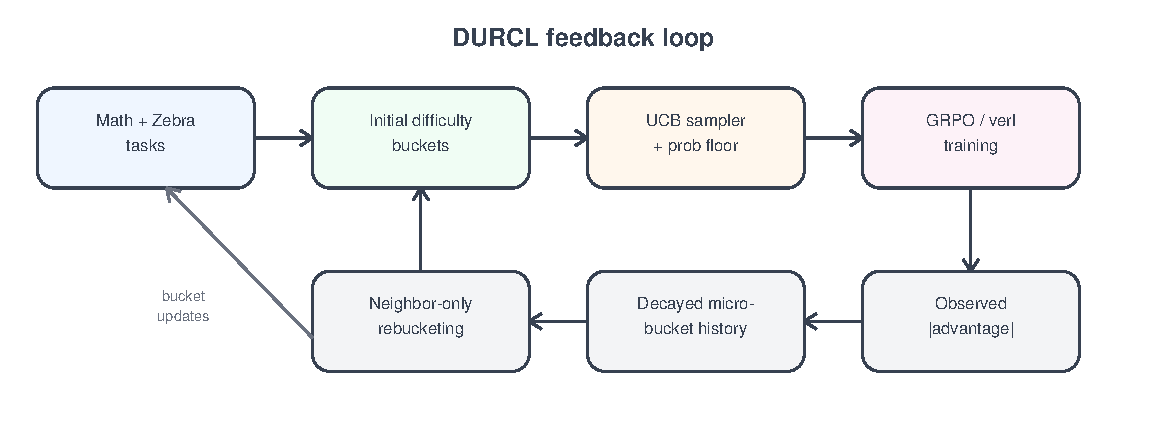
\includegraphics[width=0.96\linewidth]{figures/fig_method_pipeline.pdf}
\caption{AES feedback loop. Math and Zebra examples are placed into initial difficulty buckets. A UCB sampler selects clusters for training. Observed absolute advantages update decayed micro-bucket histories, and persistent structural mismatches are corrected through neighbor-only re-bucketing.}
\label{fig:method}
\end{figure}

\paragraph{From DUMP to AES.}
AES starts from the DUMP idea that absolute advantage can measure distribution learnability \citep{wang2025dump}. In the original DUMP algorithm, each distribution $d_j$ stores a sliding window $A^w_{d_j}$ of recent $|\hat A(o)|$ values and keeps the last $k$ entries for UCB scheduling. We make two changes for the Math+Zebra setting. First, we replace the raw sliding window with an exponential-decay state, which reduces retained statistics and gives smoother updates. Second, because Math and Zebra can drift at different learning rates, we add conservative micro-bucket re-bucketing: persistent structural mismatches may be corrected locally, allowing the curriculum structure itself to adapt instead of only changing cluster weights.

\paragraph{Initial clusters.}
The scheduler accepts explicit \texttt{cluster\_id} or \texttt{difficulty\_band} fields. It also supports a calibration map where higher measured accuracy maps to easier initial clusters. The current reported experiments mainly use coarse difficulty-based initialization, so bucket assignment is intentionally treated as imperfect.

\paragraph{Exponential-decay advantage state.}
For each sampled unit, AES maintains an exponential moving average of absolute advantage:
\begin{equation}
s_i \leftarrow \lambda s_i + (1-\lambda)|A_i|,
\end{equation}
where $\lambda$ is the decay parameter and $A_i$ is the observed advantage. Compared with a fixed-size sliding window, the decayed state requires less retained history and makes the curriculum signal smoother. Cluster values are computed from recently active advantage states.

\paragraph{UCB sampling.}
For cluster $c$, AES computes
\begin{equation}
\mathrm{UCB}_c = v_c + \beta \sqrt{\frac{2\log(N+1)}{n_c+1}},
\end{equation}
where $v_c$ is the active cluster value, $N$ is total draws, and $n_c$ is draws from cluster $c$. UCB scores are passed through a softmax and mixed with a probability floor so every nonempty cluster remains sampleable.

\subsection{Micro-bucket Rebucketing}

The cluster scheduler assumes that each curriculum cluster is internally coherent. However, this assumption can be violated when the initial clusters are built from coarse difficulty labels or noisy pre-evaluation signals. To address this, AES uses a conservative micro-bucket re-bucketing mechanism that refines cluster membership online without turning the scheduler into an unconstrained clustering algorithm.

For each initial task--cluster group, we randomly split its examples into several micro-buckets. A micro-bucket is the smallest unit allowed to move; individual samples are never moved independently. This reduces the variance of sample-level advantage estimates and makes re-bucketing a structural correction rather than an instance-level filtering procedure.

During training, each micro-bucket records the mean absolute advantage of its sampled examples. Given a recent observation window, we summarize the learning dynamics of micro-bucket $G_g$ by
\begin{equation}
z_g=(\ell_g,s_g),
\end{equation}
where $\ell_g$ is the recent average absolute advantage and $s_g$ is the fitted slope of the advantage trajectory. Thus, $\ell_g$ measures the current strength of the learning signal, while $s_g$ captures whether this signal is increasing, decreasing, or stable.

Each cluster $C_k$ also has a dynamics center, computed from the micro-buckets currently assigned to it:
\begin{equation}
z_k=\frac{1}{|\mathcal{G}_k|}\sum_{G_g\in\mathcal{G}_k}z_g.
\end{equation}
After standardizing the level and slope dimensions, a micro-bucket currently assigned to $C_k$ is compared only with $C_k$ and its adjacent clusters:
\begin{equation}
j^\star(g)=
\arg\min_{j\in\{k-1,k,k+1\}}
\|\tilde z_g-\tilde z_j\|_2^2.
\end{equation}
If the same neighboring cluster is consistently closer across multiple re-bucketing checks, the micro-bucket becomes a correction candidate.

To avoid one-way drift, the main correction operation is an adjacent mutual swap. If one micro-bucket in $C_k$ is closer to $C_{k+1}$ and another micro-bucket in $C_{k+1}$ is closer to $C_k$, AES swaps them. This keeps cluster sizes stable and prevents the re-bucketing module from replacing the scheduler. Therefore, the scheduler remains responsible for curriculum progression, while re-bucketing only corrects local structural mismatches.

\begin{algorithm}[t]
\caption{Adaptive Cluster Scheduling with Micro-bucket Rebucketing}
\label{alg:adaptive_rebucket}
\small
\begin{algorithmic}[1]
\REQUIRE Training set $\mathcal{D}$, initial clusters $\mathcal{C}=\{C_0,\ldots,C_{K-1}\}$, policy model $\pi_\theta$
\STATE Split each initial task--cluster group into micro-buckets $\{G_g\}$
\STATE Initialize cluster values $\bar A_k\leftarrow 0$ and draw counts $n_k\leftarrow 0$
\FOR{training step $t=1,\ldots,T$}
    \STATE Compute \(U_k=\bar A_k+\beta\sqrt{2\log(N+1)/(n_k+1)}\) and \(p_k=\mathrm{softmax}(U_k/\tau)\)
    \STATE Sample a cluster $C_k\sim p$ and draw a batch $B_t$ from $C_k$
    \STATE Generate rollouts with $\pi_\theta$, compute rewards, and estimate advantages $\{\hat A_i\}_{x_i\in B_t}$
    \STATE Update $\pi_\theta$ using the RL objective
    \STATE Update $\bar A_k$ and micro-bucket histories using $|\hat A_i|$
    \IF{$t\geq T_{\mathrm{warmup}}$ and $t$ is a re-bucketing checkpoint}
        \STATE For each eligible $G_g$, fit its recent dynamics signature $z_g=(\ell_g,s_g)$
        \STATE For each cluster $C_k$, compute $z_k=|\mathcal{G}_k|^{-1}\sum_{G_g\in\mathcal{G}_k}z_g$
        \STATE Standardize the level and slope dimensions of all $z_g$ and $z_k$
        \STATE For each $G_g\in C_k$, find \(j^\star(g)=\arg\min_{j\in\{k-1,k,k+1\}}\|\tilde z_g-\tilde z_j\|_2^2\)
        \STATE Mark $G_g$ if the same neighboring $j^\star(g)\neq k$ is selected consistently across checks
        \STATE For each adjacent pair $(C_k,C_{k+1})$, swap the highest-margin mutual candidates
    \ENDIF
\ENDFOR
\RETURN Fine-tuned policy $\pi_\theta$
\end{algorithmic}
\end{algorithm}

\section{Experiments}

\subsection{Step-200 Math+Zebra Validation}

The clearest positive result appears in the Math+Zebra two-task comparison. At step 200, the scheduler without re-bucketing improves over random sampling on both metrics.

\begin{figure}[H]
\centering
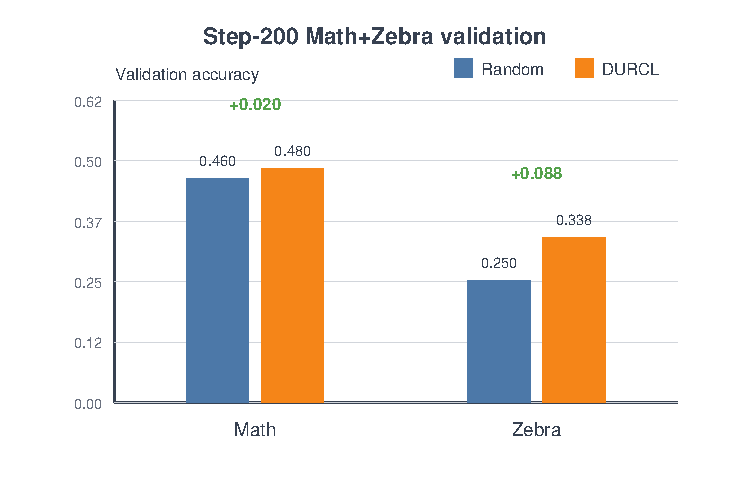
\includegraphics[width=0.58\linewidth]{figures/fig_step200_math_zebra.pdf}
\caption{Step-200 validation on Math and Zebra. The no-rebucket AES sampler improves Math by $+0.020$ and Zebra by $+0.088$ over the random baseline.}
\label{fig:step200}
\end{figure}

\begin{table}[H]
\centering
\caption{Math+Zebra step-200 validation.}
\label{tab:math_zebra}
\begin{tabular}{lccc}
\toprule
Run & Step & Math & Zebra \\
\midrule
Random baseline & 200 & 0.460 & 0.250 \\
AES sampler, no re-bucket & 200 & 0.480 & 0.338 \\
\bottomrule
\end{tabular}
\end{table}

\subsection{UCB Score Drift Diagnostic}

The UCB trace gives a mechanism-level check that the scheduler is not behaving like a fixed sampler. Figure~\ref{fig:ucb_drift} plots the five cluster scores from step 60 to step 200. These values should be read as UCB scores, not normalized probabilities. The ranking changes substantially over training: C0 decreases from 0.329 at step 60 to 0.081 at step 200, while C3 rises from 0.238 to 0.295 and C4 remains high at 0.253. In other words, early sampling pressure is concentrated on C0/C1, but later pressure shifts toward C3/C4.

This supports the claim that UCB is doing useful adaptive work: the selected clusters are changing with the estimated learner signal and the exploration term, rather than staying near the initial difficulty prior. It also exposes a drift issue. If the scores move strongly toward high-index clusters, then downstream training can be affected by the resulting cluster and task-composition shift. This is why the re-bucketing and composition diagnostics in Experiment 1 are necessary.

\begin{figure}[H]
\centering
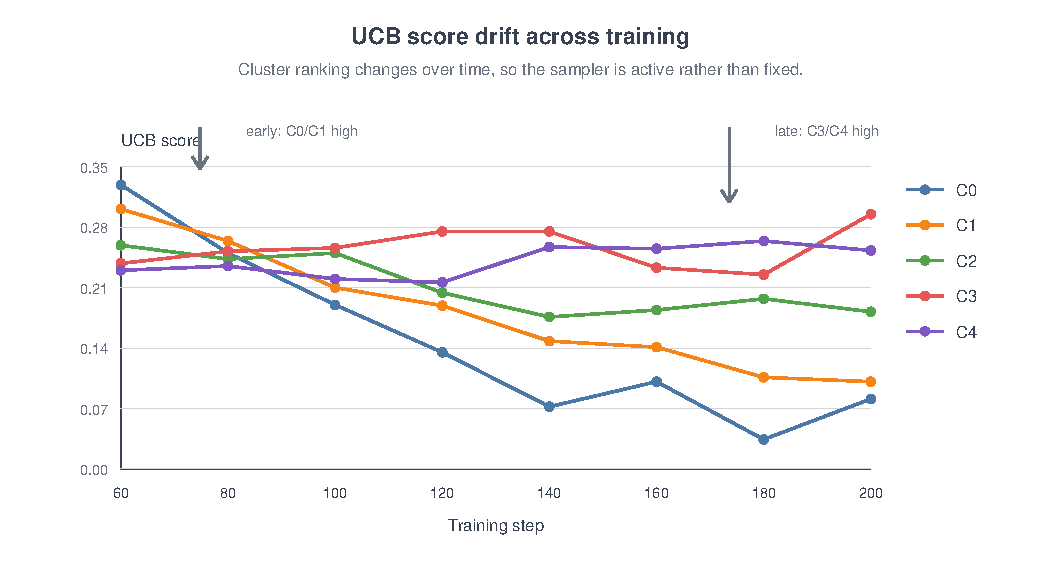
\includegraphics[width=0.72\linewidth]{figures/fig_ucb_score_drift.pdf}
\caption{UCB score drift from step 60 to step 200. Low-index clusters C0/C1 have the largest scores early, while C3/C4 dominate later. This is evidence that the UCB sampler is responsive, and it motivates monitoring drift in cluster and task composition.}
\label{fig:ucb_drift}
\end{figure}

\subsection{Experiment 1: Difficulty-Label Initialization and Composition Drift}

Experiment 1 studies whether online re-bucketing can correct imperfect initial curriculum buckets. The initial buckets are deliberately coarse: examples are initialized only from raw difficulty labels, without accuracy-based calibration. The initial accuracy test already shows why this is rough. Zebra accuracies are 0.30, 0.20, 0.25, and 0.15 for difficulties 1--4, so nominal difficulty is not strictly monotone with learner competence. Math accuracies are 0.70, 0.60, 0.35, 0.35, and 0.10 for difficulties 1--5, which is more monotone but lives on a much higher accuracy scale than Zebra. Figure~\ref{fig:init_acc} visualizes this mismatch.

\begin{figure}[H]
\centering
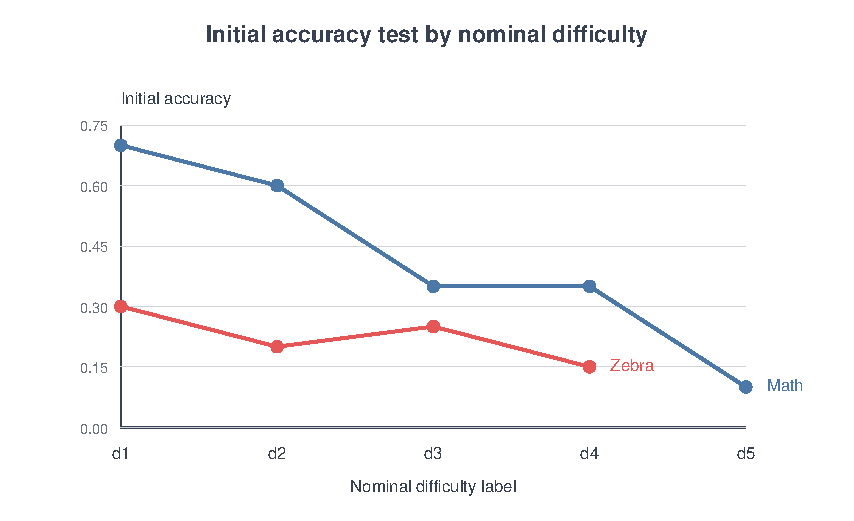
\includegraphics[width=0.58\linewidth]{figures/fig_initial_accuracy_profile.pdf}
\caption{Initial accuracy test for label-only initialization. Zebra is non-monotone across nominal difficulty labels, while Math and Zebra have different accuracy scales. This motivates accuracy-based initialization as the next step.}
\label{fig:init_acc}
\end{figure}

Even under this rough initialization, re-bucketing discovers meaningful redistribution patterns. The difficulty-init report gives a step-300 re-bucket result of 0.520 on Math and 0.287 on Zebra, compared with a baseline 200--300 reference of 0.560 on Math and 0.275 on Zebra. Thus re-bucketing is not a simple final-accuracy win; its strongest current value is diagnosing and correcting imperfect buckets. Accuracy-based initialization is the next step to test whether better initial buckets lead to cleaner and more useful corrections.

The more useful evidence is the cluster-composition shift. Figure~\ref{fig:composition} reports both micro-bucket counts and sample counts. Initially, C0--C3 each contain 5 Math and 5 Zebra micro-buckets, while C4 is already Math-only because Zebra has only four difficulty clusters but Math has five. After re-bucketing, C0 grows from 80 to 128 Math samples and 100 to 120 Zebra samples; C1 becomes Zebra-heavy, changing from 5 Math and 5 Zebra micro-buckets to 2 Math and 6 Zebra micro-buckets; C3 loses Zebra, dropping from 100 to 60 Zebra samples; and C4 remains Math-only while shrinking from 5 to 4 Math micro-buckets. This is meaningful structural correction, but it is also composition drift: AES is not merely correcting difficulty within a fixed task mixture.

\begin{figure}[H]
\centering
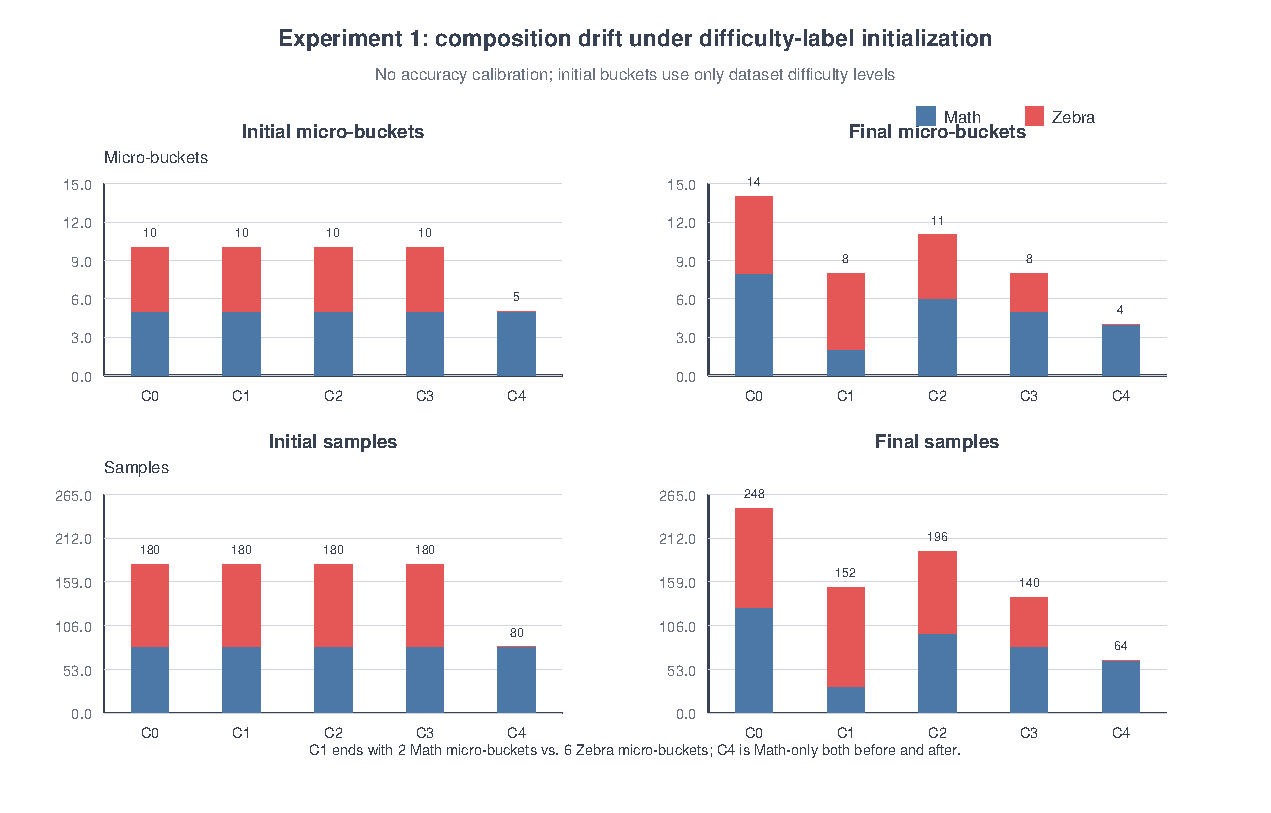
\includegraphics[width=0.92\linewidth]{figures/fig_rebucket_composition.pdf}
\caption{Experiment 1 composition drift under difficulty-label initialization. Re-bucketing changes both micro-bucket composition and sample composition: C0 grows mainly through Math inflow, C1 becomes Zebra-heavy, C3 loses Zebra, and C4 remains Math-only.}
\label{fig:composition}
\end{figure}

The direction of the net changes is also meaningful. The checked-in result summary does not include raw migration-event logs, so Figure~\ref{fig:transition} visualizes a minimal adjacent-flow interpretation of the aggregate micro-bucket changes rather than raw per-step transitions. Under this interpretation, the off-diagonal mass is adjacent and moves toward lower-index buckets: for example, Math has a large C1 $\rightarrow$ C0 flow, and Zebra has C3 $\rightarrow$ C2 flow. This is consistent with a curriculum interpretation rather than random reassignment. In particular, Math C0 expands substantially, and that bucket corresponds to the highest initial Math accuracy group.

\begin{figure}[H]
\centering
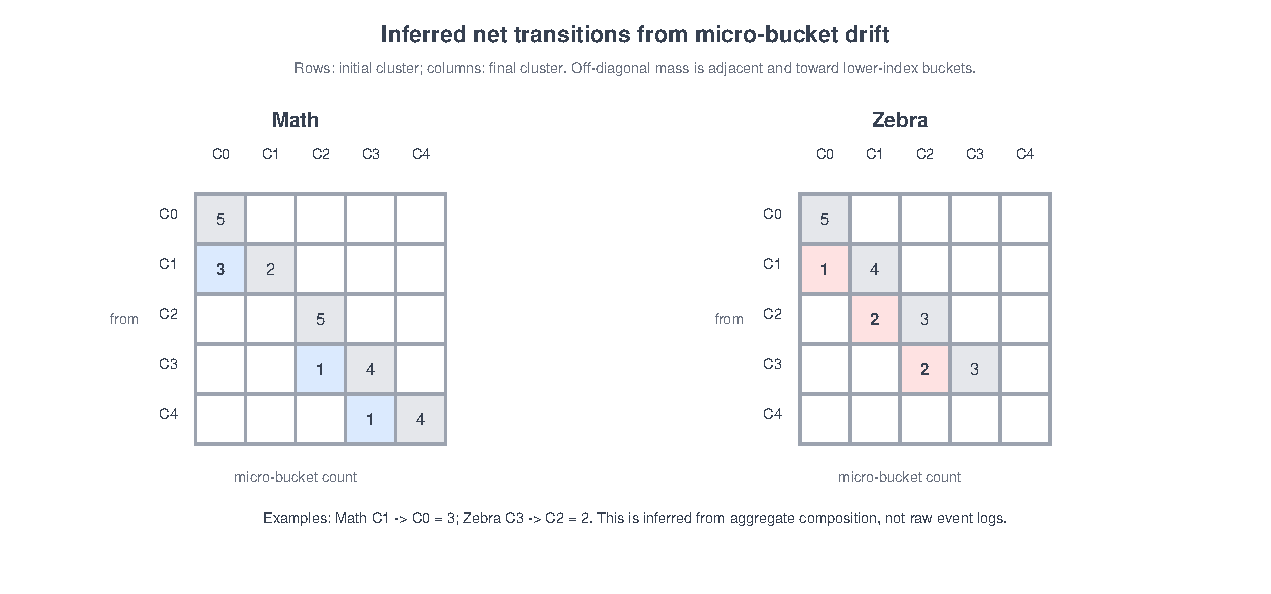
\includegraphics[width=0.82\linewidth]{figures/fig_inferred_transition_matrix.pdf}
\caption{Inferred net transition matrix from initial/final micro-bucket counts. Rows are initial clusters and columns are final clusters. The non-diagonal changes are adjacent and toward lower-index buckets, supporting the claim that re-bucketing is structured rather than random.}
\label{fig:transition}
\end{figure}

\subsection{Experiment 2: Accuracy-Based Initialization (Pending)}

The planned second experiment repeats the 200-step comparison under accuracy-based initialization. This is the direct test of the next hypothesis from Experiment 1: if the initial buckets are built from learner accuracy rather than raw difficulty labels, then re-bucketing should produce cleaner and more useful corrections. The result is not available yet, so we leave the table blank rather than inventing numbers.

\begin{table}[H]
\centering
\caption{Experiment 2 planned 200-step comparison under accuracy-based initialization. Results are pending.}
\label{tab:exp2_pending}
\begin{tabular}{lccc}
\toprule
Run & Step & Math & Zebra \\
\midrule
Acc-init, no re-bucket & 200 & pending & pending \\
Acc-init, re-bucket & 200 & pending & pending \\
\bottomrule
\end{tabular}
\end{table}

\subsection{Mechanism Check: Toy Re-Bucketing}

The toy simulation validates that migration is not triggered by ordinary drift or one-step spikes. A persistent high outlier migrates at step 300, while normal drifting and a single spike do not.

\begin{figure}[H]
\centering
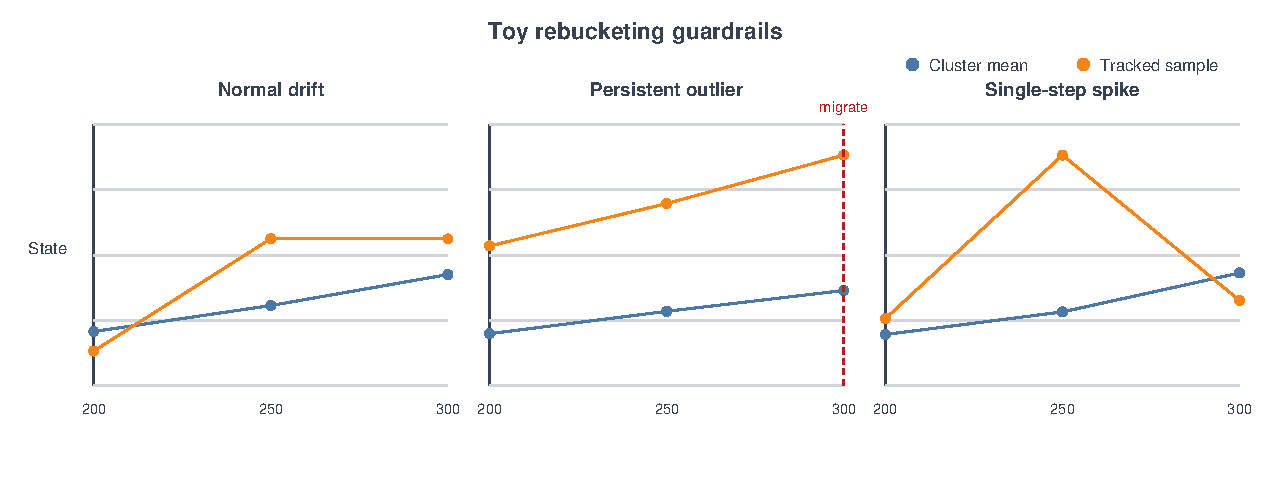
\includegraphics[width=0.96\linewidth]{figures/fig_toy_rebucket_guardrails.pdf}
\caption{Toy re-bucketing guardrails. Only the persistent outlier triggers migration; normal cluster drift and a single-step spike are filtered out.}
\label{fig:toy}
\end{figure}

\section{Discussion}

The evidence supports a conservative interpretation. AES can produce useful adaptive sampling: in the two-task result, the no-rebucket sampler improves both Math and Zebra at step 200. AES also produces interpretable structural corrections: re-bucketing moves micro-buckets in coherent ways and the toy simulation confirms the guardrails.

However, the current evidence is still limited. The re-bucketing result is stronger as a structural-correction signal than as a final-accuracy claim, and Experiment 2 under accuracy-based initialization is still pending. The composition-drift analysis also shows that micro-bucket correction can change the Math/Zebra mixture inside clusters. This suggests that the current difficulty-only initialization is not well aligned with the learner's actual state and that task-composition drift must be monitored explicitly.

The most defensible conclusion is that AES demonstrates plausible adaptive environment selection behavior in the Math+Zebra setting, but the present implementation is still an early-stage mechanism rather than a robust training recipe.

\section{Limitations and Future Work}

The current evidence is limited by single-run comparisons, missing confidence intervals, and difficulty-only initialization. Runtime artifacts such as logs and checkpoints are intentionally git-ignored, so this paper relies on checked-in summaries and CSV files rather than full run reproduction.

The highest-priority next step is accuracy-based initialization. Initial buckets should be formed from observed model pass rate per task/difficulty level, not only nominal dataset difficulty. This should reduce noisy drift and make re-bucketing corrections easier to interpret causally. Future experiments should also use multi-seed comparisons, report per-difficulty performance, add task-balance constraints or diagnostics, and separate within-task difficulty correction from cross-task composition shifts.

\section{Conclusion}

AES implements learner-state-aware environment selection for Math+Zebra RL-based LLM post-training. It combines UCB sampling, decayed advantage state, and conservative micro-bucket re-bucketing. The current results show meaningful mechanism behavior and step-200 gains over random sampling, while also revealing composition drift. The project therefore establishes a useful direction and a working implementation, while identifying accuracy-based initialization and stricter evaluation as necessary next steps.

\bibliographystyle{plainnat}
\bibliography{references}

\section*{Credit}

This report is based on the group's AES implementation, checked-in experiment summaries, and repository documentation. OpenAI Codex was used as a support tool for organizing the report draft, generating plotting scripts, formatting LaTeX text, and checking consistency with the course guideline. Core project decisions, implementation artifacts, and experimental results come from the project repository. External papers, repositories, and tools are cited in the References section.

\end{document}
